\section{Einleitung}
	\label{sec:einleitung}
	In diesem Versuch wird das Verhalten von monochromatischem Licht bei Beugung an d"unnen Spalten untersucht.\\
	Unter der Annahme, dass sich Licht wellenartig ausbreitet wird der Intensit"atsverlauf des Beugungsmusters hinter einem Einfach-, sowie einem Doppelspalt untersucht.
	Aus den Messwerten l"asst sich schlie"slich eine Aussage "uber die Spaltbreite machen.

\section{Theorie}
	\label{sec:theorie}

	Im Folgenden werden verschiedenen Annahmen gemacht, die die Beschreibung des Lichtes vereinfachen.
	Dadurch k"onnen die Ph"anomene dieses Experimentes gut erkl"art werden.

	\subsection{Das Huygenssche Prinzip}

		Um die Natur des Lichtes detailliert beschreiben zu k"onnen, muss man es quan\-ten\-me\-cha\-nisch betrachten.
		F"ur etliche Ph"anomene reicht es jedoch aus, "uber gro"se Zahlen von Lichtquanten zu mitteln und diese durch das klassische Wellenmodell n"aherungsweise zu beschreiben.
		Diese N"aherung wird hier gemacht.

		Das Huygenssche Prinzip geht von der Welleneigenschaft des Lichtes aus.
		Es besagt, dass jeder Punkt einer Wellenfl"ache zur gleichen Zeit Elementarwellen aussendet.
		Diese Kugelwellen interferieren miteinander und bilden eine neue Wellenfront,
		die die Ein\-h"ul\-len\-de der Elementarwellen ist und wiederum neue Elementarwellen aussendet.
		Die "Uberlagerung aller Elementarwellen an einem Ort im Raum beschreibt dann den dortigen Schwingungszustand der Welle.

	\subsection{Fresnel- und Fraunhoferbeugung}
		\label{subsec:beugung}

		F"ur die Beschreibung von Beugungserscheinungen gibt es grunds"atzlich zwei verschiedene Versuchsanordnungen. Abbildung \ref{abb_fresnel_fraunhofer} skizziert diese.

		\subsubsection{Fresnelbeugung}
			\label{subsubsec:fresnel}

			Die Fresnelsche Anordnung betrachtet eine Lichtquelle, die sich im endlichen Abstand vor dem Spalt befindet.
			Dadruch divergieren die Strah\-len\-b"un\-del und das Licht wird am Spalt in unterschiedlichen Winkeln gebeugt.
			Schlu"sfolgerungen auf den Versuchsaufbau durch Messung des Intensit"atsverlaufes werden damit sehr schwierig.

		\subsubsection{Fraunhoferbeugung}
			\label{subsubsec:fraunhofer}

			Diese Anordnung geht von parallelen Lichtb"undeln aus, die von einer unendlich weit entferten Lichtquelle entsandt werden.
			Hierdurch werden Lichtb"undel gleicher Phase im gleichen Winkel abelenkt.
			Die Beschreibung wird hier wesentlich einfacher, weil lediglich der Gangunterschied bei \emph{einem} Winkel, betrachtet werden muss.
			Die unendlich entfernte Lichtquelle l"asst sich gut durch einen Laser realisieren.

			Aus diesem Grund und weil der Fraunhoferaufbau eine leichtere Beschreibung der Beugung liefert, wird der Versuch damit durchgef"urt.

			\begin{figure}[h]
				\centering
				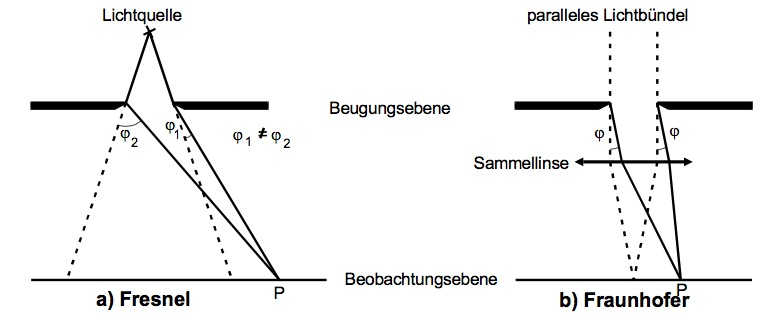
\includegraphics[width = 14cm]{fresnel_fraunhofer.jpg}
				\caption{Unterschied zwischen Fresnelschem und Fraunhoferschem 
				\newline Versuchsaufbau \cite{anleitung}}
				\label{abb_fresnel_fraunhofer}
			\end{figure}

	\subsection{Beugungsmuster am Einzelspalt}
		\label{subsec:herleitung}
		\label{subsec:muster_einzelspalt}

		\begin{figure}[h]
				\centering
				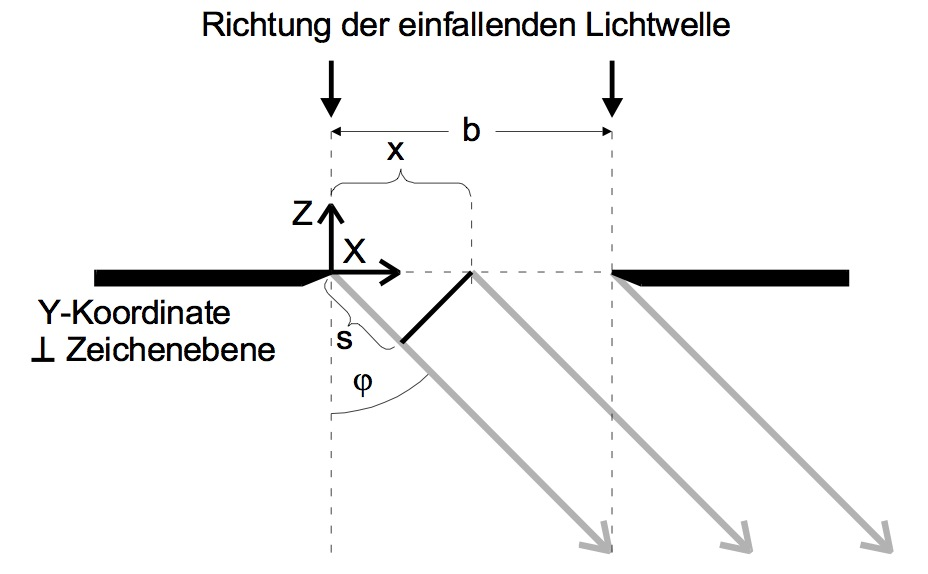
\includegraphics[width = 9cm]{spalt.jpg}
				\caption{Einzelspalt \cite{anleitung}}
				\label{abb_spalt}
		\end{figure}

		Betrachtet man nun den Spalt genauer, l"asst sich die Phasendifferenz $\delta$ zweier Strah\-len\-b"un\-del einfach beschreiben. Die durch Elementarwellen bestimmten B"undel haben dann unter dem Winkel $\varphi$ die Phasendifferenz $\delta$

		\begin{equation}
			\delta = \frac{2 \pi s}{\lambda} = \frac{2 \pi x \sin(\varphi)}{\lambda} .
		\end{equation}

		Hierbei ist $s$ gerade der Gangunterschied der B"undel und $\lambda$ die Wellenl"ange des ein\-fal\-len\-den Lichtes.\\
		Um die Amplitude $B(z, t, \varphi)$ zu bestimmen muss "uber alle Elementarwellen -- also "uber die gesamte Spaltbreite $b$ -- integriert werden:

		\begin{eqnarray}
			B(z, t, \varphi) &=& A_0 \int \limits_0^b \exp{\left[i \left(\omega t - \frac{2 \pi z}{\lambda} + \delta \right)\right]} \mathrm{dx} \nonumber \\
			&=& A_0 \exp{\left[i \left(\omega t - \frac{2 \pi z}{\lambda}\right)\right]} \int \limits_0^b \exp{\left(\frac{2 \pi i x \sin{\varphi}}{\lambda}\right)} \mathrm{dx} \nonumber\\
			\Rightarrow \enspace
			B(z, t, \varphi) &=& A_0 \exp{\left[ i \left( \omega t - \frac{2\pi z}{\lambda}
			\right) \right] } 
			\exp{\left[i \left( \frac{\pi b \sin{\varphi}}{\lambda} \right)\right]}  \cdot \nonumber \\
			&\cdot& \frac{\lambda}{\pi \sin{\varphi}}
			\sin{\left( \frac{\pi b \sin{\varphi}}{\lambda} \right)}
			.
			\label{eqn:allgemeine_lsg}
		\end{eqnarray}

		Dies beschreibt die Beugung an einem Parallelspalt.
		Die ersten beiden exponentiellen Anteile aus Gleichung \eqref{eqn:allgemeine_lsg} beschreiben die Amplitude in Abh"angigkeit der Zeit $t$ und des Ortes $z$ (senkrecht auf der Schirmfl"ache).

		Die einfallenden Lichtb"undel werden "uber lange Zeit gemessen.
		Wegen der hohen Frequenz $\omega$ des Lichtes k"onnn wir nur die "uber einige Zeit gemittelte Intensit"at $I$ messen. Der Anteil der Zeitabh"angigkeit f"allt also weg.

		Zudem bewegen wir uns lediglich entlag der Schirmfl"ache -- also in x-Richtung --, wodurch auch der zweite, z-abh"angige Term nicht betrachtet werden muss.
		Dann gilt:

		\begin{eqnarray}
			I(\varphi) & \propto & B^2(\varphi) 
		 . \nonumber
		\end{eqnarray}

		Mit einer Abk"urzung l"asst sich der Zusammenhang "ubersichtlich darstellen:

		\begin{eqnarray}
			\eta(\varphi) & := & \frac{\pi b \sin{\varphi}}{\lambda} , \nonumber \\
			\Rightarrow \qquad
			B(\varphi) & = & A_0 b \frac{\sin{\eta}}{\eta} , \label{amplitude_einfach} \\
			\Rightarrow \qquad
			I(\varphi) & \propto & A_0^2 b^2 \left(\frac{\sin{\eta}}{\eta}\right)^2  .
			\label{prop_einzelspalt}
		\end{eqnarray}

		Man erkennt, dass die H"ohe der Maxima n"aherungsweise mit dem Quadrat des Winkels abnimmt.
		Ausserdem entsteht ein Hauptmaximum bei $\varphi = 0$. Symmetrisch auf beiden Seiten entstehen etliche Nebenmaxima.
		Ein Minimum liegt vor, wenn $I(\varphi) = 0$ ist. Das gilt f"ur

		\begin{equation}
			\sin{\varphi_n} = \pm \, n \frac{\lambda}{b} \quad , \quad n = \left(1, 2, \dots\right) .
		\end{equation}

		\begin{figure}[h]
			\centering
			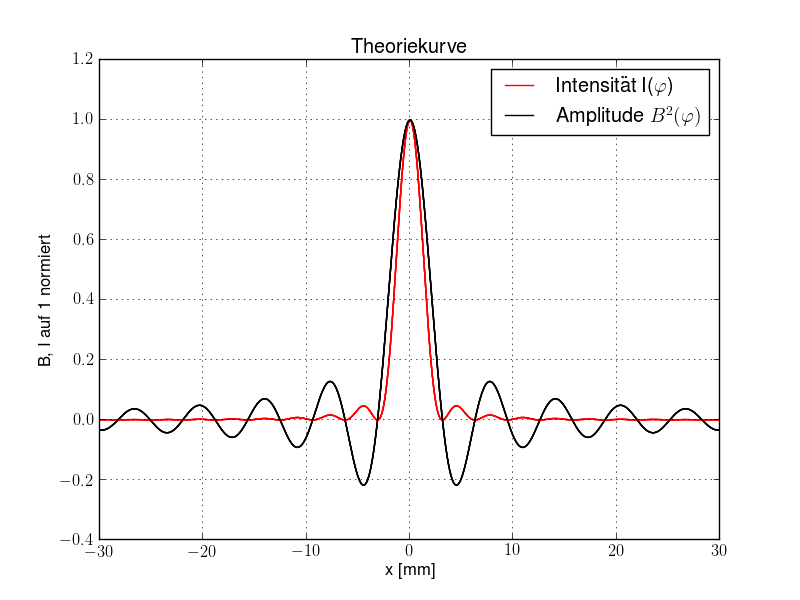
\includegraphics[height = 10cm]{theorie_1.png}
			\caption{Theoretischer Intensit"ats- und Amplitudenverlauf}
		\end{figure}

	\subsection{Fourier-Transformation}
		\label{subsec:fourier}

		Die Amplitudenverteilung l"asst sich bei diesem Aufbau auch durch eine 
		Four\-ier-Trans\-for\-ma\-tion der einzelnen Amplitudenverteilungen der einfallenden Wellen beschreiben.
		Transformiert man die Funktion $f(x)$ mit

		\begin{equation}
			f(x) = \left\{
			\begin{array}{ll}
			 	 A_0 & \qquad 0 \leq x \leq b \\
			 	 0 & \qquad \mathrm{sonst} 
			 \end{array} ,
			 \right.
		\end{equation}

		erh"alt man f"ur die Fourier-Transformation

		\begin{equation}
			g(\xi) := \int \limits_{-\infty}^{\infty} f(x) e^{ix \xi} \mathrm{dx} =
			\frac{A_0}{i \xi} \left(-1 + e^{i \xi b}\right) .
			\label{amplitude_fourier}
		\end{equation}

		Unter Anwendung der Eulerschen Formel und mit

		\begin{equation}
			g(\xi) = \frac{2 \pi \sin{\varphi}}{\lambda}
		\end{equation}

		stimmen \eqref{amplitude_fourier} und \eqref{amplitude_einfach} "uberein.
		Das Huygensche Prinzip wird hierdurch also mathematisch formuliert.
		Das Integral beschreibt dabei die Summation "uber alle Elementarwellen.
		Die Aperturfunktion $f(x)$ kann zudem hierbei einfach um eine Variable $y$ erweitert werden,
		was die Beschreibung der Beugung an zweidimensionalen Objekten erm"oglicht. \\
		F"ur die Auswertung dieses Experimentes ist besonders wichtig, dass sich die Fourier-Transformation umkehren l"asst.
		Wir k"onnen somit aus den Messwerten der Intensit"at $I(\varphi)$,
		die proportional zu $B^2(\varphi)$ ist, auf die Gestalt der Aperturfunktion $f(x)$
		--  also auf unseren Spalt -- schlie"sen.
		
	\subsection{Beugungsmuster am Doppelspalt}
		\label{sec:muster_doppelspalt}

		Der Doppelspalt l"asst sich als "Uberlagerung zweier Einzelspalte im Abstand $s$ beschreiben.
		Hieraus bekommt man zus"atzlich zur Abh"angigkeit \eqref{prop_einzelspalt} einen Cosinus-Anteil,
		der den Gangunterschied durch den Spaltabstand ber"ucksichtigt:

		\begin{equation}
			I(\varphi) \propto B^2(\varphi) = 
			4 \cos^2{\left( \frac{\pi s \sin{\varphi}}{\lambda} \right)}
			\left( \frac{\lambda}{\pi b \sin{\varphi}} \right)^2
			\sin^2{\left( \frac{\pi b \sin{\varphi}}{\lambda} \right)} .
			\label{prop_doppelspalt}
		\end{equation}

		\begin{figure}[h]
			\centering
			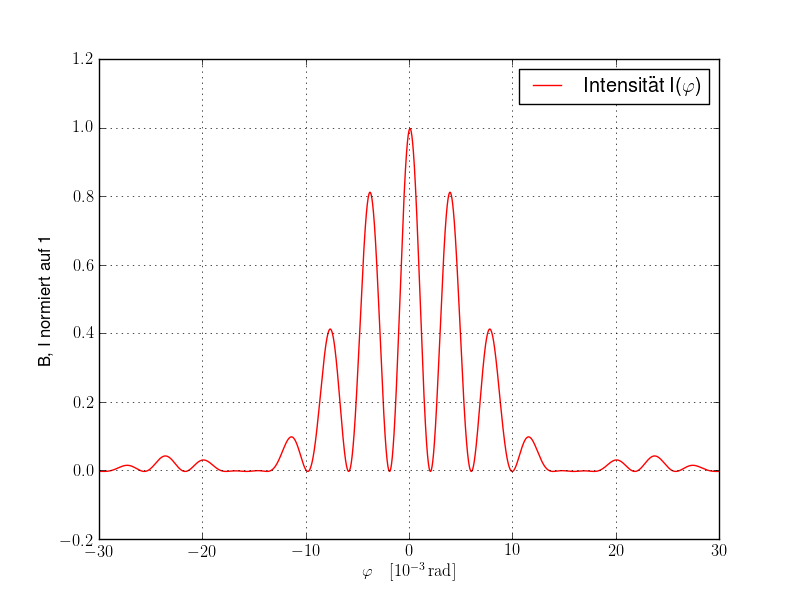
\includegraphics[width = 15cm]{theorie_2.png}
			\caption{Theoretischer Amplitudenverlauf des Doppelspaltes}
			\label{theoriekurve_doppelspalt}
		\end{figure}
